% 
% 
% Copyright (c) 2017 Valdemar Lindberg
%
% Permission is hereby granted, free of charge, to any person obtaining a copy
% of this software and associated documentation files (the "Software"), to deal
% in the Software without restriction, including without limitation the rights
% to use, copy, modify, merge, publish, distribute, sublicense, and/or sell
% copies of the Software, and to permit persons to whom the Software is
% furnished to do so, subject to the following conditions:
%
% The above copyright notice and this permission notice shall be included in all
% copies or substantial portions of the Software.
%
% THE SOFTWARE IS PROVIDED "AS IS", WITHOUT WARRANTY OF ANY KIND, EXPRESS OR
% IMPLIED, INCLUDING BUT NOT LIMITED TO THE WARRANTIES OF MERCHANTABILITY,
% FITNESS FOR A PARTICULAR PURPOSE AND NONINFRINGEMENT. IN NO EVENT SHALL THE
% AUTHORS OR COPYRIGHT HOLDERS BE LIABLE FOR ANY CLAIM, DAMAGES OR OTHER
% LIABILITY, WHETHER IN AN ACTION OF CONTRACT, TORT OR OTHERWISE, ARISING FROM,
% OUT OF OR IN CONNECTION WITH THE SOFTWARE OR THE USE OR OTHER DEALINGS IN THE
% SOFTWARE.
%
\documentclass[11pt,onsided,a4paper]{article}
\usepackage[utf8]{inputenc}
\usepackage[T1]{fontenc}
\usepackage[english]{babel}

\usepackage{listings}
\usepackage[hidelinks]{hyperref}
\lstset{basicstyle=\ttfamily,
  showstringspaces=false,
  commentstyle=\color{red},
  keywordstyle=\color{blue}
}

\thispagestyle{empty}

%
\usepackage[toc, page]{appendix}

%
\usepackage{pdfpages}
\usepackage{makecell}
\usepackage{boldline}
\pagenumbering{roman}
\usepackage{graphicx}
\usepackage{amsmath}
\usepackage{mathtools}
\usepackage{amsfonts}
\usepackage{color}
\usepackage{verbatim}
\setcounter{secnumdepth}{0} % sections are level 1
\setcounter{secnumdepth}{3}
\setcounter{tocdepth}{3}

% Make the paper look more clean.
\usepackage{titlesec}
\newcommand{\sectionbreak}{\clearpage}

\usepackage{tikz}
\usetikzlibrary{arrows,decorations.pathmorphing,backgrounds,positioning,fit,petri}
\usetikzlibrary{chains}
\usepackage{epstopdf}
\usepackage{enumitem}
%----------------------------------------------------------------------------------------
%	TITLE PAGE
%----------------------------------------------------------------------------------------

\newcommand*{\titleGM}{\begingroup % Create the command for including the title page in the document
\hbox{ % Horizontal box
\hspace*{0.2\textwidth} % Whitespace to the left of the title page
\rule{1pt}{\textheight} % Vertical line
\hspace*{0.05\textwidth} % Whitespace between the vertical line and title page text
\parbox[b]{0.75\textwidth}{ % Paragraph box which restricts text to less than the width of the page

{\noindent\Huge\bfseries ATDB \\[0.3\baselineskip] \textit{\text{Attiny Development Board}} }% Title
{\large \textit{Documentation of the board features and board layout.}}\\[4\baselineskip] % Tagline or further description
{\Large \textsc{Valdemar Lindberg }} % Author name

\vspace{0.5\textheight} % Whitespace between the title block and the publisher
{\noindent  }\\[\baselineskip] % Publisher and logo
}}
\endgroup}


\begin{document}


%\pagestyle{empty} % Removes page numbers
\thispagestyle{empty}
\titleGM % This command includes the title page

\pagenumbering{arabic}%
\tableofcontents
\newpage


\section{Introduction}

\emph{RS232-RGB-LED-Controller} is a lightweight cheap RGB LED controller board for computer motherboards, using the \emph{COM-Port} as the main interface, which is a common, non used port on motherboards.

The controller is powered with an \emph{Atmel Atmega8AU} micro-controller, running at 16 MHZ that handles the communication between the external devices.

%
The controllers schematic and board layout was designed with the \emph{Autodesk Eagle} software under the \emph{OPHW} license. Whereas the source code for the firmware and driver is under the \emph{GPL} license. 


%
\subsection{Features}

\noindent\rule{\textwidth}{1pt}

\begin{enumerate}

\item Debug - JTAG interface easy debugging.
\\

\item Peripheral Features: RS232
\\
\item Speed Grade:
\\
\item Operating Voltage: 
	5.0V
\\
\item RGB
\\
\item Power Consumption at 1MHz, 1.8V,% 25\°C
\\
\end{enumerate}

%
\section{Pin Configurations}

\subsection{Pin-out}
Figure \ref{fig:pinout}. 12-pin PDIP

\begin{figure}[!h]
\centering 
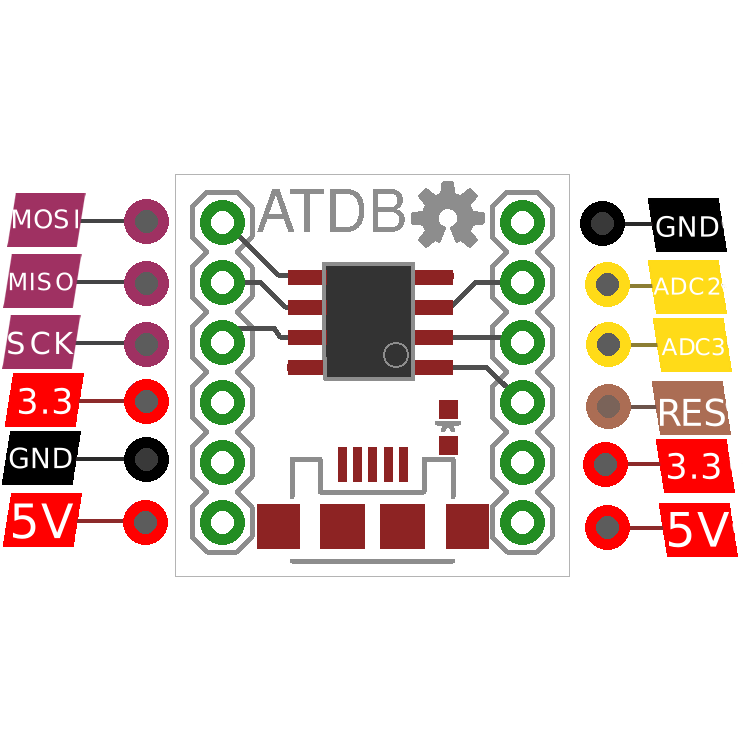
\includegraphics[width=0.75\textwidth]{outline.png}
\caption{Ouput pin of the controller}
\label{fig:pinout}
\end{figure}

\subsection{Pin Description}\label{sec:pindesc}

\newpage
\section{Schematic}
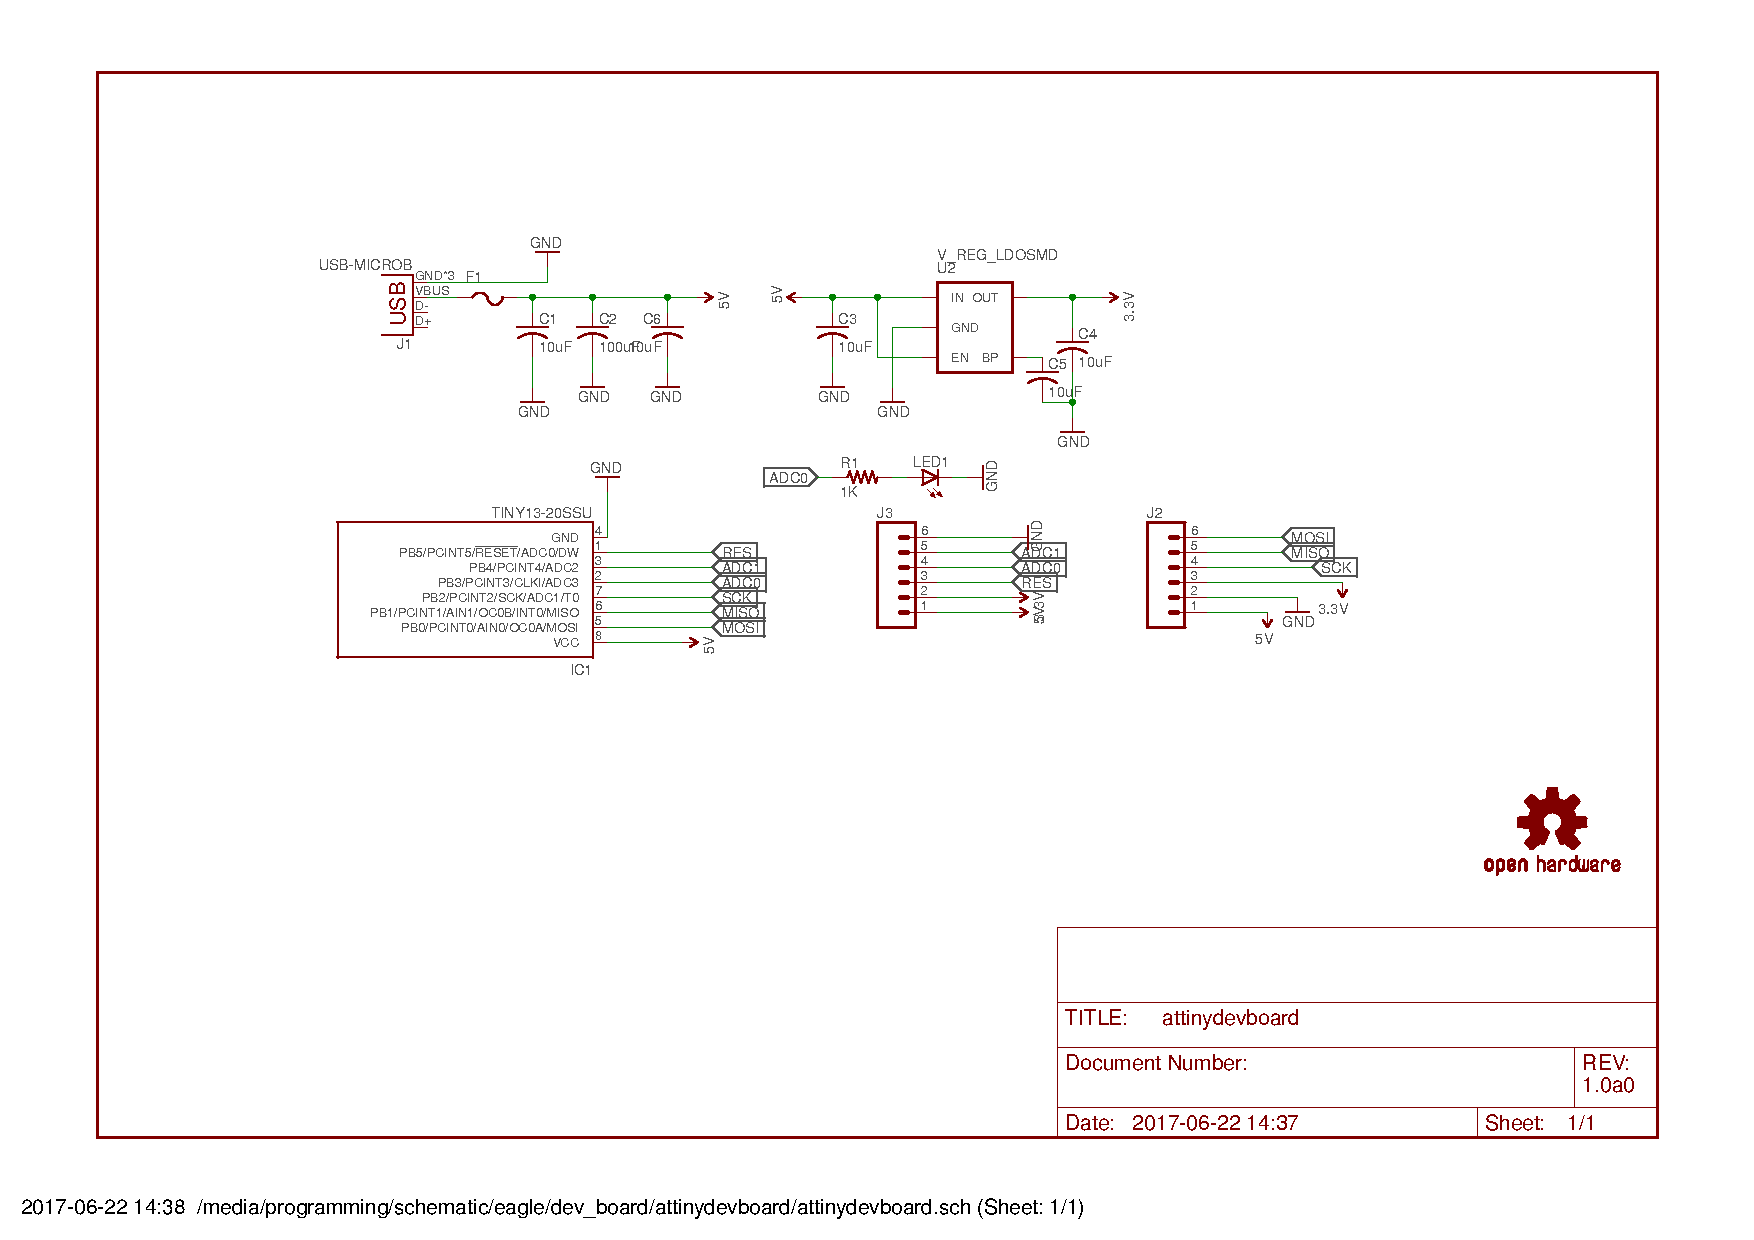
\includepdf[pages={1}, angle=90, nup=1x3]{schematic.pdf}

\end{document}
